% Formelsammlung fuer Dynamische Systeme, 2014/15
% based on template from www.latex4ei.de
% 2 Seiten

% Dokumenteinstellungen
% ======================================================================
\documentclass[german]{latex4ei/latex4ei_sheet}

\setlist{nosep}

\newcommand{\os}[2]{\ensuremath{\overset{#1}{#2}}}

\title{Dynamische Systeme}

% Dokumentbeginn
% ======================================================================
\begin{document}

\IfFileExists{git.id}{\input{git.id}}{}
\ifdefined\GitRevision\mydate{\GitNiceDate\ (git \GitRevision)}\fi

\maketitle

\section{Grundlagen}
\begin{sectionbox}
Zustands-DGL: $\underline{\dot{x}} =  \underline{f}\left( \underline{x}, \underline{u}, t \right) $ \\
Ausgangsgleichung: $\underline{y} = \underline{h} \left( \underline{x}, \underline{u}, t \right)$ \\
$\underline{x} \in \mathbb{R}^n$, $\underline{u} \in \mathbb{R}^m$, $\underline{y} \in \mathbb{R}^q$, $t \in \mathbb{R}$\\

Steuerungsaffin: $\underline{\dot{x}} = \underline{f}(\underline{x}) + \sum_{i=1}^{m} \underline{g_i}(\underline{x}) u_i$

\begin{equation*}
\text{Jacobi-Matrix:} \,
\left[ \frac{\partial f_i}{\partial x_j} \right] =
\begin{bmatrix}
  \frac{\partial f_1}{\partial x_1} &   \cdots  &   \frac{\partial f_1}{\partial x_n} \\
  \vdots                            &           &   \vdots \\
  \frac{\partial f_n}{\partial x_1} &   \cdots  &   \frac{\partial f_n}{\partial x_n}
\end{bmatrix}
\end{equation*}
\end{sectionbox}

\begin{sectionbox}
\subsection{Linearisierung um eine Referenzlösung}

Referenzlösung: $\underline{x}^*(t), \underline{y}^*(t), \underline{u}^*(t), t > 0$ \\

Linearisierung: \\
$\underline{\dot{x}}^* + \Delta\underline{\dot{x}} = \underline{f}\left( \underline{x}^*, \underline{u}^* \right) +
\left[ \frac{\partial f_i}{\partial x_j} \right]_{(x^*, u^*)} \Delta\underline{x} +
\left[ \frac{\partial f_i}{\partial u_j} \right]_{(x^*, u^*)} \Delta\underline{u}
$

Kleinsignalmodell:
\begin{align*}
  \Delta \underline{\dot{x}}    &=  \left[ \frac{\partial f_i}{\partial x_j} \right]_{(x^*, u^*)} \Delta\underline{x} +
                                    \left[ \frac{\partial f_i}{\partial u_j} \right]_{(x^*, u^*)} \Delta\underline{u} \\
  \Delta \underline{{y}}        &=  \left[ \frac{\partial h_i}{\partial x_j} \right]_{(x^*, u^*)} \Delta\underline{x} +
                                    \left[ \frac{\partial h_i}{\partial u_j} \right]_{(x^*, u^*)} \Delta\underline{u}
\end{align*}

\begin{align*}
  \text{Standardform:} \,
  \Delta \underline{\dot{x}}    &=  A(t) \Delta\underline{x} + B(t) \Delta\underline{u} \\
  \Delta \underline{y}          &=  C(t) \Delta\underline{x} + D(t) \Delta\underline{u}
\end{align*}
\end{sectionbox}

\begin{sectionbox}
\subsection{Linearisierung um eine Ruhelage}

Ruhelage: $\underline{\dot{x}}^* = \underline{f}\left( \underline{x}^*, \underline{u}^*, t \right) = \underline{0}$

\begin{align*}
  \text{Standardform:} \,
  \Delta \underline{\dot{x}}    &=  A \Delta\underline{x} + B \Delta\underline{u} \\
  \Delta \underline{y}          &=  C \Delta\underline{x} + D \Delta\underline{u}
\end{align*}

\subsection{Lokale Existenz und Eindeutigkeit einer Lösung von $f(x,x_0,t)$}

\begin{itemize}
  \item Wenn $f$ Lipschitz-stetig ist
  \item Lipschitz-stetigkeit schwer zu überprüfen, deshalb anderes Kriterium:
    \begin{enumerate}
      \item $f$ ist stetig
      \item $f$ ist stetig diff'bar
    \end{enumerate}
\end{itemize}

\subsection{Gültigkeitsbereich von Eigenschaften}
Hyperball: $\mathcal{B}_\varepsilon = \left\{ x \in \mathbb{R}^n | \|x-x^*\| \leq \varepsilon \right\}$ \\
Eigenschaft gilt:
\begin{itemize}
  \item lokal, wenn sie für alle $x \in \mathcal{B}_\varepsilon$ gilt
  \item global, wenn sie für alle $x \in \mathbb{R}^n$ gilt
  \item uniform, wenn sie für alle $t_0 \geq 0$ gilt
\end{itemize}
\end{sectionbox}

\begin{sectionbox}
\subsection{Definitheit von Funktionen}

\subsubsection{Positiv definite Funktionen (pdf)}
\begin{tabular}{cccc}
  $V(x) > 0$ & für & $x \neq 0$ & und \\
  $V(x) = 0$ & für & $x = 0$ &
\end{tabular}

\subsubsection{Positiv semidefinite Funktionen (psdf)}
\begin{tabular}{cccc}
  $V(x) \leq 0$ & für & $x \neq 0$ & und \\
  $V(x) = 0$ & für & $x = 0$ &
\end{tabular}

\subsubsection{Negativ (semi)definite Funktionen}
\begin{tabular}{cccc}
  negativ definit: & $-V(x)$ ist pd \\
  negativ semidefinit: & $-V(x)$ ist psd
\end{tabular}

\subsubsection{Lipschitz-Stetigkeit}
$\exists L \geq 0 : \| f(x,t) - f(y,t) \| \leq L \cdot \|x-y\| $
\end{sectionbox}

\begin{sectionbox}
\subsubsection{Stabilität im Sinne von Lyapunov (iSvL)}
Ruhelage $x^* = 0$ ist:
\begin{itemize}
  \item stabil: $\|x(t_0)\| < \delta \Rightarrow \|x(t)\| < \varepsilon$
  \item asymptotisch stabil: $\|x(t_0\| < \delta \Rightarrow \lim\limits_{t \rightarrow \infty} \|x(t)\| = 0 = x^*$
  \item uniform stabil: $\|x(t_0)\| < \delta \Rightarrow \|x(t)\| < \varepsilon, \forall t \geq t_0$
  \item uniform asymptotisch stabil: $x^*$ ist uniform stabil und \\ $\|x(t_0)\| < \delta \Rightarrow \lim\limits_{t \rightarrow \infty} \|x(t)\| = 0$
  \item instabil: $x^*$ ist nicht stabil
\end{itemize}

\subsubsection{Lie-Ableitung von $V(x)$}
$\dot{V}(\underline{x}) = \sum\limits_{i=1}^{n} \frac{\partial V}{\partial x_i}f_i(x) = \frac{\partial V}{\partial \underline{x}} \underline{f}(\underline{x}) $

\subsubsection{Lie-Ableitung}
$L_f h := \nabla h \cdot f$

\subsubsection{Mehrfache Anwendung der Lie-Ableitung}
$L_f^0 h = h$ \\
$L_f^i h = L_f L_f^{i-1} h$

\subsubsection*{Lie-Klammern}
$\left[ f,g \right] = \frac{\partial g}{\partial x} f - \frac{\partial f}{\partial x} g = L_f g - L_g f$

\subsubsection*{ad-Operator}
$\text{ad}_f^0 g = g(x)$ \\
$\text{ad}_f^i g = \left[ f, \text{ad}_f^{i-1} g \right]$

\subsubsection*{Ruhelage bestimmen}
$\dot x = f(x,t) \overset{!}{=} 0$
\end{sectionbox}

\section{Harmonische Balance}
\begin{sectionbox}
\subsection{Periodisches Verhalten}

Lösungstrajektorie: $\underline{\Phi}$

Grenzzyklus: $\underline{x}_G(t)$

Menge aller Punkte auf dem Grenzzyklus: $\left\{ \underline{x}_G \right\}$

Lösungstrajektorie ist periodisch\\ $ \Leftrightarrow \underline{\Phi}\left( (t+T), t_0, \underline{x}_0 \right) = \underline{\Phi}\left( t,t_0,x_0 \right)$

Kleinster Abstand $\rho$: $\rho\left( x(t), \left\{ x_G \right\} \right) = \min\limits_{ \left\{ x_G \right\} } \|x(t) - x_G(t)\| $

Bahnstabilität: $\left\{ x_G \right\}$ ist bahnstabil $\Leftrightarrow$:
$\exists \varepsilon > 0, \delta(\varepsilon) > 0: \rho(x_0, \left\{ x_G \right\}) < \delta(\varepsilon) \Rightarrow \rho(x(t), \left\{ x_G \right\}) < \varepsilon$

$\Rightarrow$ Anfangsabstand $\rho_0 < \delta(\varepsilon)$, dann Abstand immer $< \varepsilon$

\subsection{Asymptotische Bahnstabilität}

\begin{enumerate}
  \item $\left\{ x_G \right\}$ bahnstabil
  \item $\lim\limits_{t \rightarrow \infty} \rho\left( x(t), \left\{ x_G \right\} \right) = 0 $
\end{enumerate}
$\Rightarrow$ Trajektorie $x(t)$ geht auf Grenzzyklus $x_G(t)$ zu, $\forall x \in \mathbb{R}^n$

\subsection{Asymptotisch semistabil}
$\Rightarrow$ Trajektorie $x(t)$ geht nur für bestimmte Menge an Punkten $\in \mathbb{R}^n$ auf $x_G(t)$ zu.
\end{sectionbox}

\begin{sectionbox}
\subsection{Existenz von Grenzzyklen in planaren Systemen}
\begin{emphbox}
\begin{align*}
  \text{im $\mathbb{R}^2$:} \,
  \dot{x}_1 =&  f_1(x_1, x_2) \\
  \dot{x}_2 =&  f_2(x_1, x_2)
\end{align*}
\end{emphbox}

\subsubsection{Benedixson-Kriterium}
Hat div$\left\{ \underline{f}(x_1, x_2) \right\}$ keine Vorzeichenänderung in $\mathcal{M}$, dann gibt es keinen Grenzzyklus in $\mathcal{M}$ \\
mit $\text{div}\left\{ \underline{f}(x_1, x_2) \right\} = \left[ \frac{\partial f_1}{\partial x_1} + \frac{\partial f_2}{ \partial x_2} \right]$

\subsubsection{$\omega$-Limit-Set}

$\lim\limits_{n \rightarrow \infty} \underline{\Phi} (t_n, t_0, x_0) = \underline{z}$ \\
Menge aller Punkte $z$ heißt $\omega$-Limit-Set
\end{sectionbox}

\begin{sectionbox}
\subsection{Methode der Harmonischen Balance}

System besteht aus Kennlinie $f(e, \text{sgn}(\dot{e}))$ und Teilsystem $G(j\omega)$. \\
Voraussetzungen:
\begin{itemize}
  \item An Blöcke:
    \begin{itemize}
      \item $f(.)$ ist punktsymmetrisch
      \item $G(j\omega)$ ist LTI und hat hinreichenden Tiefpass-Charakter (d.h. relativer Nennegrad < 2)
    \end{itemize}
  \item eingeschwungen
  \item $e(t)$ bzw $y(t)$ sind näherungsweise harmonisch \\ (d.h. $e(t) = A \sin(\omega t) = \text{Re} \left\{ -j A e^{j\omega t} \right\}$)
\end{itemize}

\subsubsection{Gleichung der Harmonischen Balance bzw Schwingbedingung}
\begin{emphbox}
  $N(A) \cdot G(j\omega) = -1$
\end{emphbox}
mit Beschreibungsfunktion $N(A) = \frac{a_1 + j b_1}{A}$ \\
inverse Beschreibungsfunktion $N_I(A) = - \frac{1}{N(A)}$ \\

\begin{cookbox}{Vorgehen zum Koeffizienten-Bestimmen}
  \item $a_1, b_1$:  $u(t)$ fourier-transformieren zu $\bar{u}(t)$ \\
    $\Rightarrow a_1 = \frac{2}{T_0} \int\limits_{T_0} u(t) \sin(\omega t) \diff t; \\
                 b_1 = \frac{2}{T_0} \int\limits_{T_0} u(t) \cos(\omega t) \diff t$
  \item $A$: $e(t) = A \sin(\omega t)$, bzw wird berechnet als $A_g$ mit $\omega_g$
\end{cookbox}

\subsubsection{Bestimmen von $A_g, \omega_g$}
\begin{cookbox}{algebraisch}
  \item Aus Gleichung der Harmonischen Balance folgt: $N(A)G(j\omega) = -1$ bzw. $G(j \omega) = N_I(A)$
  \item $\text{Re}\left\{ G(j \omega) \right\} = \text{Re} \left\{ N_I(A) \right\}$
  \item $\text{Im}\left\{ G(j \omega) \right\} = \text{Im} \left\{ N_I(A) \right\}$
\end{cookbox}

\begin{cookbox}{geometrisch}
  \item $G(j \omega)$ und $N_I(A)$ in komplexer Ebene aufzeichnen
  \item bei Schnittpunkten gilt: $G(j \omega) = N_I(A)$
  \item Schnittpunkte sind mögliche Grenzschwingungen
  \item $\Rightarrow$ algebraisch $A_g$ und $\omega_g$ bestimmen
\end{cookbox}

\subsubsection{Stabilität von Grenzschwingungen, graphisch bestimmen}
Nyquistkriterium bzgl kritischen Punktes $N_I(A_g)$ anwenden
\end{sectionbox}

\section{Stabilität nichtlinearer Systeme}
\begin{sectionbox}

\subsection{Direkte Methode von Lyapunov}
Damit kann Stabilität, aber keine Instabilität nachgewiesen werden

\subsubsection{Zeitinvariante Systeme}

\subsubsection{Direkte Methode von Lyapunov für lokale Stabilität}

$x^*$ ist \underline{lokal} (asymptotisch) stabil iSvL wenn:
\begin{itemize}
  \item $x^*$ ist Ruhelage
  \item $V(x)$ ist stetig diff'bar
  \item $V(x)$ ist \underline{lokal} pd
\end{itemize}
\begin{tabular}{cccc}
  wenn  &$\dot{V}(x) \leq 0 \Rightarrow$& lokal stabil \\
   &$\dot{V}(x) < 0 \Rightarrow $& lokal asymptotisch stabil
\end{tabular}

\subsubsection{Direkte Methode von Lyapunov für globale Stabilität}

$x^*$ ist \underline{global} (asymptotisch) stabil iSvL wenn:
\begin{itemize}
  \item $x^*$ ist Ruhelage
  \item $V(x)$ ist stetig diff'bar
  \item $V(x)$ ist \underline{global} pd
  \item $V(x)$ ist radial unbeschränkt (dh $\|x\| \rightarrow \infty \Rightarrow V(x) \rightarrow \infty$
\end{itemize}
\begin{tabular}{cccc}
  wenn  &$\dot{V}(x) \leq 0 \Rightarrow$& global stabil \\
   &$\dot{V}(x) < 0 \Rightarrow $& global asymptotisch stabil
\end{tabular}

\subsubsection{Zeitvariante Systeme}
Notwendige Bedingungen damit $x^*$ lokal uniform (asymptotisch) stabil ist:
\begin{itemize}
  \item $x^*$ ist Ruhelage
  \item $V(x)$ ist stetig diff'bar
\end{itemize}

\subsubsection{Lokale Stabilität}
$x^*$ ist lokal uniform stabil iSvL wenn:
\begin{itemize}
  \item $W_1(x), W_2(x)$ stetig pdf
  \item $W_1(x) \leq V(x,t) \leq W_2(x)$
  \item $\dot{V}(x,t) = \frac{\partial V}{\partial t} + \frac{\partial V}{\partial \underline{x}} \underline{f}(x,t) \leq 0$
\end{itemize}

$x^*$ ist lokal uniform asymptotisch stabil wenn zusätzlich gilt:
\begin{itemize}
  \item $W_3(x)$ stetig, lokal pdf
  \item $\dot{V}(x,t) = \frac{\partial V}{\partial t} + \frac{\partial V}{\partial \underline{x}} \underline{f}(x,t) \leq -W_3(x)$
\end{itemize}

\subsubsection{Globale Stabilität}
Uniforme Stabilität ist global wenn zusätzlich gilt: \\
$V(x,t)$ ist radial unbeschränkt
\end{sectionbox}

\begin{sectionbox}
\subsection{Häufig verwendete Lyapunov-Funktionen und deren Eigenschaften}
$V(x,t) = \dots$
\begin{itemize}
  \item $\|x\|^2$: pdf, abnehmend, radial unbeschränkt
  \item $x^T P x, P \in \mathbb{R}^{n \times n}$,pdf: pdf, abnehmend, radial unbeschränkt
  \item $(t+1) \|x\|^2$: pdf, radial unbeschränkt
  \item $e^{-t}\|x\|^2$: pdf, abnehmend
  \item $\sin^2(\|x\|^2)$: lokal pdf, abnehmend
\end{itemize}

\subsection{Exponentielle Stabilität}
$x^* = 0$ ist exponentiell stabile Ruhelage wenn folgende äquivalente Aussagen gelten:
\begin{itemize}
  \item $c,m,\alpha > 0 $ existieren für alle $\|x(t_0)\| < c$ so dass: $\|x(t)\| \leq me^{-\alpha(t-t_0)}$
  \item $\alpha_1, \alpha_2, \alpha_3, \alpha_4 > 0$ existieren so dass:\\
    $\alpha_1 \|x\|^2 \leq V(x,t) \leq \alpha_2 \|x\|^2$ \\
    $\dot{V}(x,t) \leq - \alpha_3 \|x\|^2$ \\
    $\|\frac{\partial V(\underline{x},t)}{\partial \underline{x}}\| \leq \alpha_4 \|x\| $
\end{itemize}
\end{sectionbox}

\begin{sectionbox}
\subsection{Invarianzprinzip von LaSalle}
Invarianzmenge $\mathcal{M}: x(t_0) \in \mathcal{M} \Rightarrow  x(t) \in \mathcal{M}, \forall t \geq t_0$

\subsubsection{Invarianzprinzip}
\begin{itemize}
  \item $\Omega$ ist kompakte(dh abgeschlossen und beschränkt) Invarianzmenge
  \item $V(x)$ stetig diff'bar und $\dot{V}(x) \leq 0$ auf $\Omega$
  \item $\varepsilon \subseteq \Omega$ mit $V(\varepsilon) = 0$
  \item $\mathcal{M} \subseteq \varepsilon$, $\mathcal{M}$ ist größte Invarianzmenge in $\varepsilon$
\end{itemize}
$\Rightarrow$ jede Lösung die in $\Omega$ beginnt, nähert sich $\mathcal{M}$ an für $t \rightarrow \infty$ \\
daraus folgt: \\
Besteht $\mathcal{M}$ nur aus $\underline{0}$ und ist $\dot{V}(x) \leq 0$, dann \\
$\Rightarrow$ Ruhelage $\underline{0}$ ist asymptotisch stabil

\subsubsection{Korollar: Barbashin}
\begin{itemize}
  \item $x^*$ ist Ruhelage
  \item $V(x)$ ist stetig diff'bar und pdf auf $\mathcal{B}_\varepsilon$
  \item $\dot{V}(x) \leq 0$ auf $\mathcal{B}_\varepsilon$
  \item $\mathcal{S} := {x \in \mathcal{B}_\varepsilon | \dot{V}(x) = 0 }$
\end{itemize}
Wenn nur $x(t)=0$ in $\mathcal{S}$ bleiben kann, dann ist $x^* = 0$ asymptotisch stabil

\subsubsection{Korollar: Krasovski (globale Variante von Barbashin)}
\begin{itemize}
  \item $x^*$ ist Ruhelage
  \item $V(x)$ ist stetig diff'bar, pdf und radial unbeschränkt auf $\mathbb{R}^n$
  \item $\dot{V}(x) \leq 0$ auf $\mathbb{R}^n$
  \item $\mathcal{S} := {x \in \mathbb{R}^n | \dot{V}(x) = 0 }$
\end{itemize}
Wenn nur $x(t)=0$ in $\mathcal{S}$ bleiben kann, dann ist $x^* = 0$ global asymptotisch stabil
\end{sectionbox}

\begin{sectionbox}
\subsection{Indirekte Methode von Lyapunov}
\subsubsection{Zeitinvariante Systeme}
Linearisierung um Ruhelage $x^*$:\\
Systemmatrix $A = \left[ \frac{\partial \underline{f}(\underline{x})}{\partial \underline{x}} \right]_{x=x^*}$
\begin{itemize}
  \item $A$ ist negativ definit $\Rightarrow x^*$ ist lokal asymptotisch stabil
  \item $A$ ist indefinit oder positiv (semi-)definit $\Rightarrow x^*$ ist lokal instabil
  \item $A$ ist negativ semidefinit $\Rightarrow$ keine Aussage über $x^*$ möglich
\end{itemize}

\subsubsection{Zeitvariante Systeme}
Linearisierung um Ruhelage $x^*$ \\
$\Rightarrow \dot{x} = A(t) x + f_1(x,t)$, wobei \\
\begin{itemize}
  \item $A(t) = \left[ \frac{\partial f(x,t)}{\partial x} \right]_{x=x^*}$
  \item $f_1(x,t)$ Restterm
\end{itemize}

Bedingung: Vereinfachte Linearisierung $\dot{x}  = A(t) x$ gültig falls: \\
$\lim\limits_{\|x\| \rightarrow 0} \sup\limits_{t \geq 0} \frac{\|f_1(x,t)\|}{\|x\|} = 0$

Stabilität des nichtlinearen Systems
\begin{itemize}
  \item $x^*$ ist uniform asymptotisch stabil in Linearisierung \\
    $\Rightarrow x^*$ ist uniform asymptotisch stabil im nichtlinearen System
  \item $x^*$ ist instabil in Linearisierung \\
    $\Rightarrow$ keine Aussage über $x^*$ im NL System möglich
  \item $x^*$ ist instabil in Linearisierung und $A(t) = A_0 = const$ \\
    $\Rightarrow x^*$ instabil im NL System
\end{itemize}

\subsubsection{Stabilität von LTV Systemen(1)}
Ruhelage des LTV Systems ist exponentiell stabil wenn
\begin{itemize}
  \item $\left[ A(t) + A(t)^T \right]$ negativ definit ist für alle $t$
  \item $A(t)$ negativ definit ist und $A(t)$ beschränkt ist, dh $\int\limits_{0}^{\infty}A(t)^T A(t) \diff t < \infty$
\end{itemize}

\subsection{Instabilität}
Falls Stabilität nicht nachgewiesen werden kann, versucht man Instabilität nachzuweisen

\subsubsection{Satz von Chetaev}
\begin{itemize}
  \item $x^* = 0$ ist Ruhelage
  \item $V(x)$ ist stetig diff'bar, $V(0)=0, V(x_0)>0$ für $\|x_0\| > 0$
  \item $\mathcal{U} := \left\{ x \in \mathcal{B}_\varepsilon | V(x) > 0 \right\}$
\end{itemize}
Wenn $\dot{V}(x) > 0$ auf $\mathcal{U}$, dann ist $x^*=0$ instabil

Bemerkung:
\begin{itemize}
  \item $V(x)$ muss keine pdf sein
  \item Es genügt Menge $\mathcal{U}$ zu finden, so dass: $V(x) > 0$ und $0 \in \mathcal{U}$
\end{itemize}
\end{sectionbox}

\begin{sectionbox}
\subsection{Einzugsgebiet}
Falls asymptotisch stabile Ruhelage nicht global asymptotisch stabil \\
$\Rightarrow$ Einzugsgebiet bestimmen, in der die Ruhelage lokal asymptotisch stabil ist

\subsubsection{Einzugsgebiet, Domain of Attraction, Basin}
$\mathcal{A}(x^*) := \left\{ x_0 | \lim\limits_{t \rightarrow \infty} \Phi(t,t_0,x_0) = x^* \right\}$ \\
mit $\Phi(t,t_0,x_0)$ als Lösung der DGL

\subsubsection{Bestimmen des Einzugsgebiets}
\begin{itemize}
  \item $x^*$ ist Ruhelage, asymptotisch stabil
  \item $\mathcal{V} = {x^*} \cup \left\{ x | V(x) > 0, \dot{V}(x) < 0 \right\}$
  \item $\mathcal{E}_c = \left\{ x | V(x) \leq c \right\}$
\end{itemize}
Wenn $\mathcal{E}_c \subseteq \mathcal{V}$ und $\mathcal{E}_c$ ist beschränkt, dann ist $\mathcal{E}_c$ Teilmenge des Einzuggebiets

\subsection{Lyapunov-basierter Reglerentwurf}
\begin{cookbox}{Vorgehen}
  \item $V(x)$ so aufstellen, dass $u$ in $V(x)$ und in $\dot{V}(x)$ vorkommt
  \item $u$ so einstellen, dass $V(x) > 0$ und $\dot{V}(x) < 0$
\end{cookbox}
\end{sectionbox}

\section{Passivität}
\begin{sectionbox}
Achtung: $V(x)$ ist abstrakte Speicherfunktion \\
Energiespeicherfunktion zB. aus physikalischer Energiebetrachtung\\

Verallgemeinerte Energiebilanz und Versorgungsrate eines Systems:
\begin{emphbox}
$\int\limits_{0}^{t} s(u,y) \diff \tau + V(x(0)) = \int\limits_{0}^{t} g(\tau) \diff \tau + V(x(t))$
\end{emphbox}
\begin{tablebox}{ll}
Netto-Energiezufluss & $\int\limits_{0}^{t} s(u,y) \diff \tau$ \\
Versorgungsrate & $s(u,y)$ \\
Anfangs gespeicherte Energie & $V(x(0))$ \\
dissipierte Energie & $\int\limits_{0}^{t} g(\tau) \diff \tau$ \\
dissipierte Leistung & $g(\tau)$ \\
gespeicherte Energie & $V(x(t))$ \\
\end{tablebox}
Es gilt $\int\limits_{0}^{t}|s(u(\tau), y(\tau))| \diff \tau < \infty$

\subsubsection{Dissipativität (dissipativ bzgl $s(u,y)$)}
$V(x)$ ist psdf \\
Integrale Dissipativitätsungleichung: $\int\limits_{0}^{t} s(u,y) \diff \tau + V(x(0)) \geq V(x(t))$ \\
Differentielle Dissipativitätsungleichung: $s(u,y) \geq \dot{V}(x(t))$

\subsubsection{Passivität}
Dissipativ bzgl spezieller Versorgungsrate $s(u,y) = y^T u$ \\
$V(x)$ ist psdf \\
Integrale Passivitätsungleichung: $\int\limits_{0}^{t} y^T u \diff \tau + V(x(0)) \geq V(x(t))$ \\
Differentielle Passivitätsungleichung: $s(u,y) \geq \dot{V}(x(t))$ \\
\begin{tabular}{cccc}
  streng passiv: &  $\Rightarrow$ bei '$>$' & bzw $g(t) > 0$ \\
  verlustlos:    &  $\Rightarrow$ bei '=' & bzw $g(t) = 0$
\end{tabular}
\end{sectionbox}

\begin{sectionbox}
\subsection{Passivität und Stabilitätseigenschaften}

\subsubsection{Passivität und Lyapunov-Stabilität}
\begin{itemize}
  \item System ist passiv
  \item $V$ ist stetig diff'bar und psd
\end{itemize}
$\Rightarrow$ Ruhelage $x=0$ ist stabil iSvL

\subsubsection{Null-Zustandsbeobachtbarkeit}
Nur $x^*=0$ kann in $\mathcal{S} = \left\{ x \in \mathbb{R} | h(x,0)=0 \right\}$ bleiben

\subsubsection{Passivität und asymptotische Stabilität}
$x^*=0$ ist asymptotisch stabil wenn eine der beiden Punkte zutrifft:
\begin{itemize}
  \item System ist streng passiv
  \item über $V(x)$:
    \begin{itemize}
      \item System ist passiv
      \item $V(x)$ ist stetig diff'bar und pdf
      \item $\dot{V}(x) = 0 \Leftrightarrow y = 0$
      \item Null-Zustand beobachtbar
    \end{itemize}
\end{itemize}

Wenn $V(x)$ zusätzlich radial unbeschränkt ist $\Rightarrow x^* = 0$ ist global asymptotisch stabil
\end{sectionbox}

\section{Passivitätsbasierte Regelung}
\begin{sectionbox}
$x^* = 0$ ist global asymptotisch stabil\\
$\Rightarrow$ System kann stabilisiert werden mit $u = -\Phi(y)$, wobei:
\begin{itemize}
  \item $\Phi$ ist lokal Lipschitz-stetig
  \item $\Phi$ ist beliebig
  \item $\Phi(0) = 0$
  \item $y^T \Phi > 0$ für $y \neq 0$
\end{itemize}

\begin{tabular}{cccc}
mögliche $\Phi$:  & $\Phi = k_i \text{sat}(y_i)$ & \\
                  & $\Phi = \frac{2 k_i}{\pi}\text{atan}(y_i)$ &
\end{tabular}

\subsubsection{Feedback-Passivierung}
Ziel: Nicht-Passive Systeme in passive transformieren durch spezielle Wahl der Ausgangsfunktion $y=h(x)$ \\
$\dot{x} = f(x) + G(x)u$ \\
$\Rightarrow$ Ausgang $y = h(x) \overset{\text{def}}{=} \left[ \frac{\partial V}{\partial x} G \right]^T$ \\
Ist Ausgang dann Null-Zustandsbeobachtbar $\Rightarrow$ es kann global stabilisierendes Regelgesetz gefunden werden
\end{sectionbox}

\section{Feedback-Linearisierung}
\begin{sectionbox}
\begin{cookbox}{Nichtlineare System-Transformation: $z = \varphi (x)$}
  \item Zustandstransformation: $z = \varphi(x)$
  \item NL-RNF aufstellen
  \item Überprüfen ob $\varphi(x)$ ein Diffeomorphismus ist
  \item Feedback-linearisierendes Regelgesetz aufstellen
\end{cookbox}

\subsubsection{Nichtlineare Regelungsnormalform, NL-RNF}
\begin{align*}
  \dot{z}_1 &= z_2 \\
  \dot{z}_2 &= z_3 \\
            &\dots \\
  \dot{z}_n &= a(x) + b(x) u \\
\end{align*}

\subsubsection{Diffeomorphismus}
$z = \varphi(x)$ ist (lokal) gültige Zustandstransformation wenn $\nabla \underline{\varphi}$ nicht singulär ist, $\Leftrightarrow \det(\nabla \varphi) \neq 0$ \\
$\nabla \underline{\varphi} = \left[ \frac{\partial \varphi_i}{\partial x_j} \right]$, Jacobi-Matrix

\subsubsection{Feedback-linearisierendes Regelgesetz}
$u(x) = \frac{1}{b(x)}[v - a(x)]$ \\
$\Rightarrow \dot{z}_n = v $
\end{sectionbox}

\section{E/A-Linearisierung}
\begin{sectionbox}
\begin{cookbox}{Vorgehen}
  \item Ausgang $y$ festlegen, dessen dynamische Antwort auf Reglereingang $v$ linearisiert werden soll
  \item Zeitliche Ableitung des Ausgangs $y$ liefert nach einigen Schritten  die E/A-Beziehung in RNF
  \item Aus RNF das feedback-linearisierende Regelgesetz aufstellen
  \item Bei Bedarf Systemtransformation durchführen, so dass $\dot{z}_n = v$
\end{cookbox}

$\dot{x} = f(x) + g(x)u$ \\
$\Rightarrow \dot{y}(x) = \frac{\partial h}{\partial x}f(x) + \frac{\partial h}{\partial x}g(x)u = L_f h(x) + L_g h(x) u$ \\

\subsubsection{zu 2.}
$y$ so lange ableiten bis: $\overset{(r)}{y} = a(x) + b(x) u$ \\
\begin{align*}
  \dot{y}           &= L_f h                            &(\text{mit} L_g h(x) = 0) \\
  \ddot{y}          &= L_f^2 h                          &(\text{mit} L_g L_f h(x) = 0) \\
                    &\dots                              & \\
  \overset{(r)}{y}  &= L_f^r h + L_g L_f^{r-1} h(x) u   &
\end{align*}

\subsubsection{zu 3.}
$u(x) \overset{!}{=} \frac{1}{b(x)} [v - a(x)]$ \\
Neuer virtueller Systemeingang: $v = \overset{r}{y}$ \\
Regelgesetz: $u(x) = \frac{v - L_f^r h(x)}{L_g L_f^{r-1} h(x)}$

\subsubsection{Relativer Grad bzw Differenzengrad}
\begin{tablebox}{ll}
Vollstandige Linearisierung & $r = n$ \\
interne Dynamik vorhanden & $r < n$ \\
Nulldynamik & $y(t) = 0, \forall t$, mit interner Dynamik
\end{tablebox}
\end{sectionbox}

\begin{sectionbox}
\subsection{Zustands-Linearisierung}
$\dot{x} = f(x) + g(x)u$ \\
$\dot{z} = \nabla \varphi(x) \left( f(x) + g(x)u \right)$
\begin{cookbox}{Vorgehen}
  \item Nichtlineare Zustandstransformation bestimmen $\Rightarrow \varphi(x)$
  \item Regelgesetz bestimmtn
\end{cookbox}

\subsubsection{zu 1.}
GLS lösen: \\
\begin{align*}
  \underbrace{
  \begin{bmatrix}
    g^T \\
    [\text{ad}_f g]^T \\
    \vdots \\
    [\text{ad}^{n-2}_f g]^T \\
    [\text{ad}^{n-1}_f g]^T \\
  \end{bmatrix}
  }_{S^T}
  \left[ \frac{\partial \varphi_1(x)}{\partial x} \right]^T
  =
  \begin{bmatrix}
    0 \\
    0 \\
    \vdots \\
    0 \\
    g^*
  \end{bmatrix}
\end{align*}

Matrix $S$ ist Erreichbarkeitsmatrix \\

GLS ist gleichbedeutend mit: \\
$ L_g L_f^i \varphi_1(x) =
\begin{cases}
  0, & i = 0, \dots, n-2 \\
  \hat{g}^*(x), & i = n-1
\end{cases}$

ist gleichbedeutend mit: \\
$\left[ \frac{\partial \varphi_1(x)}{\partial x} \right] \text{ad}_f^i g(x) =
\begin{cases}
  0, & i = 0, \dots, n-2 \\
  \hat{g}(x), & i = n-1
\end{cases}$

wobei:\\
$\hat{g}^*, g^* \neq 0$ \\
$g* = (-1)^{n-1} \hat{g}^*$\\

Dann nach $\frac{\partial \varphi_1}{\partial x}$ auflösen und daraus $\varphi_1$ bestimmen. \\
Für die restlichen $\varphi_i$ gilt: $\varphi_i(x) = L_f^i \varphi_1$

\subsubsection{zu 2.}
Regelgesetz: $u(x) = \frac{1}{L_g L_f^{n-1} \varphi_1(x)} \left( v - L_f^n \varphi_1(x) \right)$\\
wobei $v$: neuer Regeleingang
\end{sectionbox}

\section{Flachheitsbasierte Regelung}
\begin{sectionbox}
\begin{cookbox}{Vorgehen}
  \item Flachheitsanalyse
  \item Flachheitsbasierte Steuerung
  \item Flachheitsbasierte Folgeregelung
\end{cookbox}

\subsubsection{zu 1. Flachheitsanalyse}
System ist flach wenn folgende Bedingungen erfüllt sind:
\begin{itemize}
  \item es gibt (fiktiven) Ausgang $y = \Phi(x, u, \dot{u}, \dots, \os{(\alpha)}{u})$ \\
    mit dim $y$ = dim $u$
  \item eine (lokal) eindeutige Zustandsfunktion kann gefunden werden: \\
    $x = \Psi_1 (y, \dot{y}, \dots, \os{(\gamma)}{y})$
  \item eine (lokal) eindeutige Eingangsfunktion kann gefunden werden: \\
    $u = \Psi_2 (y, \dot{y}, \dots, \os{(\gamma +1)}{y})$
\end{itemize}

\begin{cookbox}{Flachen Ausgang bestimmen}
  \item Ausgang sollte möglichst viel Information über das dynamische Systemverhalten haben
  \item Sukzessive zeitliche Ableitung des Kandidaten zur Herleitung von Gleichungen zur Bestimmung von $x$ und $u$
  \item $y$ muss so oft abgeleitet werden, bis aus dem resultierenden GLS von $y,\dots,\os{\gamma}{y}$ alle unbekannten $x$ und $u$ (lokal) bestimmt werden können
  \item Kandidat ist umso erfolgversprechender, je häufiger abgeleitet werden kann ohne dass Eingänge $u$ auftauchen
\end{cookbox}

Danach $x = \Psi_1 (y, \dot{y}, \dots, \os{(\gamma)}{y})$ und $u = \Psi_2 (y, \dot{y}, \dots, \os{(\gamma +1)}{y})$ bestimmen

\subsubsection{zu 2. Flachheitsbasierte Steuerung}
\begin{cookbox}{Solltrajektorie bestimmen}
  \item $y_d$ bestimmen: entweder vorgegeben oder\\
    falls $y_d$ nicht vorgegeben, dann aus $x_d$ oder Regelgröße $w$ bestimmen
  \item zugehörige $x_d$ und $u_d$ bestimmen
\end{cookbox}

\subsubsection{zu 3. Flachheitsbasierte Folgeregelung}
\begin{cookbox}{Zustandsrückführung und Nichtlineares Regelgesetz aufstellen}
  \item fiktive (differentierte) Ausgänge $\left[ y, \dots, \os{(\alpha)}{y} \right]$ als Eingänge $v$ einführen
  \item Nichtlineares Regelgesetz aufstellen: $u = \Psi\left( y, \dots, \os{(\alpha)}{y}, v \right)$
  \item Zustandstransformation: $z = \dots$
  \item Zustands-DGL: $\dot{z} = \dots$
\end{cookbox}
\end{sectionbox}

\section{Backstepping}
\begin{sectionbox}
\subsection{Anwendungsgebiet}
$u \rightarrow \dot{x}_n \rightarrow \int \dots \rightarrow \dot{x}_i \rightarrow \int \rightarrow \dot{x}_1 \rightarrow \int \rightarrow x_1$

\begin{align*}
  \dot{x}_1 &=      & f_1(x_1) + g_1(x_1)x_2 \\
  \dot{x}_2 &=      & f_2(x_1, x_2) + g_2(x_1, x_2)x_3 \\
            &\vdots & \\
  \dot{x}_i &=      & f_i(x_1, \dots, x_i) + g_i(x_1, \dots, x_i)x_{i+1} \\
            &\vdots & \\
  \dot{x}_n &=      & f_n(x_1, \dots, x_n) + g_n(x_1, \dots, x_n)u
\end{align*}
\end{sectionbox}

\begin{sectionbox}
\subsection{Verfahren (rekursiv anwenden)}
System wird in Teilsysteme unterteilt. Ausgang des einen Teilsystems ist Pseude-Stellgröße des nachfolgenen Systems.

\begin{cookbox}{Vorgehen}
  \item Transformiertes Teilsystem aufstellen\\
    $z = \dots$\\
    $\dot{z} = \dots$
  \item Pseudo-Stellgröße festlegen
  \item Partielle Lyapunov Funktion aufstellen:
    \begin{itemize}
      \item  Meist:\\
        $V_1 = \frac{1}{2} z_1^2$\\
        $V_i = V_{i-1} + \frac{1}{2}z_i^2$ \\
        $V_n = \frac{1}{2} \sum\limits_{i=1}^{n} z_i^2$
      \item $\dot{V}_i = \Psi(z, x_{i+1}) \Rightarrow x_{i+1}$ so festlegen, dass $\dot{V}_i^* < 0$
    \end{itemize}
  \item Funktion für gewünschte Stellgröße $\alpha_i$ bestimmen: $x_{i+1} := \alpha_i$
  \item So lange rekursiv anwenden bis $\alpha_i = u$
\end{cookbox}
\end{sectionbox}

\section{Sliding Mode Regelung}
\begin{sectionbox}
System: $\dot{x} = f(x) + g(x)u + d(t)$ \\
wobei $d(t)$ unbekannte Störfunktion ist \\
Schaltmannigfaltigkeit: $S = \left\{ x \in \mathbb{R}^n | s(x) = 0 \right\}$ \\
unstetige Stellgröße:
$u(x) =
\begin{cases}
  u^+(x) & \text{für} s(x) > 0 \\
  u^-(x) & \text{für} s(x) < 0 \\
\end{cases}$\\
unstetiges Systemverhalten:
$\dot{x} =
\begin{cases}
  f^+(x) & \text{für} s(x) > 0 \\
  f^-(x) & \text{für} s(x) < 0 \\
\end{cases}$\\
Regelziel: Systemzustand soll nach ersten Kontakt auf Schaltmannigfaltigkeit $s(x) = 0$ bleiben\\
Gezielte Unterdrückung von Störung ist möglich wenn:
\begin{itemize}
  \item $d(x,t)$ liegt in dem von $g(x)$ aufgespannten Raum
  \item $|d_i| < D_i, D_i = const \in \mathbb{R}$
\end{itemize}

\begin{cookbox}{Vorgehen}
  \item Diskontinuierliche Reglerfunktion finden, so dass System in endlicher Zeit in den Sliding Mode geht\\
  Um in den Sliding Mode zu kommen muss gelten:
  \begin{itemize}
    \item $s_i \dot{s}_i < 0$
    \item $\lim\limits_{s_i(x) \rightarrow 0^\pm} \dot{s}_i(x) = k^{\mp} \lessgtr 0$
  \end{itemize}
  \item Schaltmannigfaltigkeit so wählen, dass im Sliding Mode gewünschte Systemdynamik auftritt (Beschreibung des Systemverhaltens $\dot{x}$)
\end{cookbox}

\subsubsection{zu 1.}


\subsubsection{Idealer Sliding Mode nach Filippov}
$\dot{x} = f(x)$\\
Ansatz: $\dot{x}_\text{fi} = \alpha f^+(x) + (1-\alpha) f^-(x)$ mit $0 \leq \alpha \leq 1$ \\
Bedingung: $\dot{s}(x_\text{fi}) = \frac{\partial s}{\partial x} \dot{x}_\text{fi} = 0$ \\
Man erhält: $\alpha = \frac{ \frac{\partial s}{\partial x} f^-(x)  }{ \frac{\partial s}{\partial x} (f^-(x) - f^+(x))  }$ \\
und somit:\\ $\dot{x}_\text{fi} = \frac{ \frac{\partial s}{\partial x} f^-(x)  }{ \frac{\partial s}{\partial x} (f^-(x) - f^+(x)) } f^+(x) -
\frac{ \frac{\partial s}{\partial x} f^+(x)  }{ \frac{\partial s}{\partial x} (f^-(x) - f^+(x)) } f^-(x)$ \\
Wobei: $\frac{\partial s}{\partial x}f^- \geq 0$ und $\frac{\partial s}{\partial x}f^+ \leq 0$ \\

\subsubsection{Idealer Sliding Mode nach der Equivalent Control Method}
$\dot{x} = f(x) + g(x)u$ \\
Es gilt: $s(x) = 0, \dot{s}(x) = 0$ \\
Daraus folgt: $\dot{s}(x) = L_f s(x) + L_g s(x) \tilde{u}_\text{eq}$ \\
Kontinuierliche Ersatzstellgröße: $\tilde{u}_\text{eq} = -L_g s(x) ^{-1} L_f s(x)$ \\
Systemdynamik: $\dot{x} = f(x) - g(x) L_g s(x)^{-1} L_f s(x)$
\end{sectionbox}

\begin{sectionbox}
\subsection{Blockschaltbild}
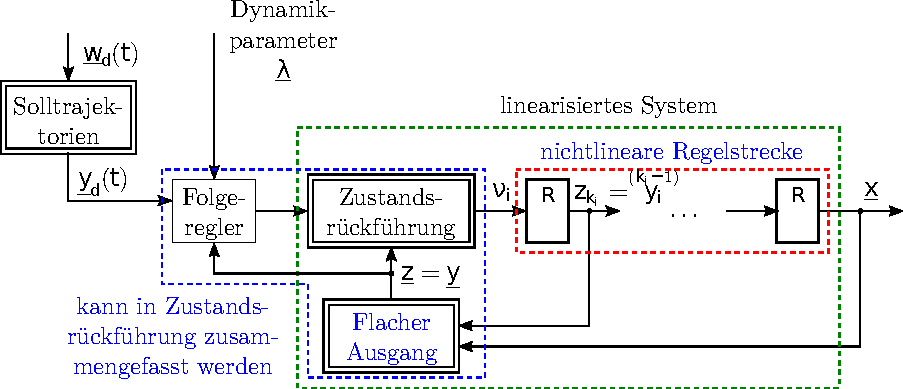
\includegraphics[angle=90, width=5cm]{./img/block.pdf}
\end{sectionbox}

\end{document}
